\documentclass[11pt]{book}
\usepackage{basecommon}
\usepackage[margin=1.5in, top=1in]{geometry}
\usepackage{graphicx}
\usepackage[backend=bibtex, natbib=true, autocite=superscript, style=authoryear-ibid]{biblatex}
\usepackage{hyperref}
\usepackage{url}
\usepackage{lineno}
\usepackage{fancyhdr}
\renewcommand{\familydefault}{ppl} % try phv, ptm, ppl
\addbibresource{citations_annotated.bib}
\graphicspath{ {images/} }
\usepackage{setspace}
\doublespacing
\title{Chapter 1 (DRAFT)}
\author{Hugh Zabriskie}
\date{7 March 2016}

% Fix for ToC page numbering
\fancypagestyle{plain}{%
\fancyhf{} % clear all header and footer fields
\fancyhead{} % clear all header fields
\fancyfoot{} % clear all footer fields
\fancyhead[RO]{\thepage}
\fancyhead[LE]{\thepage}
\renewcommand{\headrulewidth}{0pt}
\renewcommand{\footrulewidth}{0pt}
}


\begin{document}

% Title
\begin{titlepage}
	\centering
	{\par}
	\vspace*{3.5cm}
	{\Large\bfseries\center J.S. BOT: Exploring Computational Harmonic Analysis and Prediction in the Bach Chorales\par}
	\vspace{3.5cm}
	{by Hugh P. Zabriskie '16\par}
	\vspace{5cm}
	{submitted in partial fulfillment of the requirements for an AB degree with honors in Computer Science and Music\par}
	\vspace{1.5cm}
	{Departments of Computer Science and Music\par}
	{Harvard College\par}
	\vspace{0.5cm}
	{March 7, 2016\par}
	\vfill
\end{titlepage}

% Display page numbers in the headings. Start with roman numerals %
% Preface materials have roman numerals %
\setcounter{page}{1}
\pagenumbering{roman}
\pagestyle{fancy}
\renewcommand{\headrulewidth}{0pt}
\fancyhf{}
\fancyhead[R]{\thepage}

% Abstract
\vspace*{3cm}
{\Large\bfseries\centering Abstract \par}
\vspace*{1cm}
{The Baroque composer J.S. Bach harmonized over 300 chorale melodies over his lifetime, which today remain a pivotal body of music in the history of Western music and exemplify Bach's groundbreaking compositional techniques. Bach's harmonizations establish a series of compositional conventions that musicians today continue to emulate in order to learn 4-part counterpoint. By transforming the Chorales into a numerical dataset, this thesis examines the ability of a variety of machine learning models to learn perform harmonic analysis over the chorale melodies as well as generate new and stylistically appropriate harmonizations. \par}
\vspace*{1cm}
{An introduction to the core theoretical concepts is provided in Chapter 1 as a foundation for the interdisciplinary research conducted in this thesis. Chapters 2 and 3 explains the methods and results for the non-neural and neural models, respectively, demonstrating the ability of both model types to effectively analyze and generate chorale harmonizations. Chapter 4 seeks to generalize these findings and explore the task of contrapuntal melodic generation, focusing on the two-voice counterpoint in Bach's Inventions. \par}
{ \par}
\newpage


% Acknowledgements
\begin{center}
\vspace*{4cm}
{\Large\bfseries Acknowledgements \par}
\vspace*{2cm}
To be completed.
\end{center}
\newpage

% Table of contents
\tableofcontents
\newpage

% Add line numbers
\linenumbers

% Add headers
\pagestyle{fancy}
\fancyhf{}
\renewcommand{\headrulewidth}{0.5pt}
\rhead{\thepage}

% Start page counting back at 1
\setcounter{page}{1}
\pagenumbering{arabic}
\chapter{A Theoretical Overview}

This thesis examines the potential for algorithmic models to learn the processes and conventions involved in harmonizing a chorale melody that Bach pioneered centuries ago. One objective of this work is to improve upon previous computational attempts at chorale harmonization by consistently incorporating musical knowledge about the Chorales and the general approach to harmonizing a melody into the major design decisions of the research. By thoughtfully extracting musical features, we hope  the f  is to take advantage of musical knowledge of the Chorales to thoughtfully extract features and develop a more suited model. \\

The purpose of this chapter is to provide a high-level introduction to the topics in the music and computer science fields that are relevant to this thesis. The highly interdisciplinary nature of this research requires a certain level of familiarity with both the fundamentals of music theory and counterpoint, as well as the mathematical mechanisms that drive the machine learning models used in later chapters.

\section{An introduction for the musician}


\subsection*{Supervised machine learning}

Supervised learning is a general task in machine learning concerned with learning outcomes based on observations from a dataset. Machine learning can be broadly divided into two categories, supervised and unsupervised learning, which are defined by their different learning objectives. Unsupervised learning involves examining datasets for pattern or statistical structures that define the dataset. There are no explicit outcomes specified, so an unsupervised learning algorithm has no sense of the "correct" answer. In contrast, a supervised learning model is trained to correlate observations from a data set with a corresponding set of outcomes. Given a dataset of observations and outcomes, the model can learn to predict future outcomes. Consider the task of learning to predict the price of a car given a set of information that describes the car's features (i.e. color, year manufactured, etc.). In supervised learning, the model observes several cars and their known prices, and then updates it parameters in order to more accurately predict other car prices based on the data it has observed. Therefore, the primary task is to optimize the model's \textit{parameters}, denoted by the symbol $\theta$, in order to improve accuracy of predictions. In algebraic terms, $\theta$ is often a $n$-dimensional array of parameters such that our prediction is modeled as $h(x) \sim \theta^T x$. During training, the model updates its parameters based on a cost function - a metric for calculating the error between the predicted outcome and the known outcome - in order to reduce error for future predictions.

\subsection*{Distributions and classification}

The models used in this thesis are classifiers, meaning that they accept a vector of input features - or a series of input vectors - and for each input, it outputs a corresponding \textit{distribution}. In logistic regression and other classification algorithms, the possible outcomes or values of $y$ represent a discrete set of $k$ classes, and the distribution produced by the algorithm represents the probability that $\boldx$ belongs to each class. These distributions are initially unknown, but the objective is to learn to estimate these distributions given a dataset of observations and known outcomes. Mathematically, the objective is to learn the mapping $f: {\mathcal X} \rightarrow {\mathcal Y}$, given a set of $n$ examples, such that $h(\boldx) \approx \boldy$, where $\boldx$ is an individual input vector. The training data is the subset of the original data on which the model learns $h(\boldx)$ by updating its parameters, and the model's ability to predict future outcomes is measured based on a test set.

\subsection*{Logistic regression}

Logistic regression is a binary (2-class, \{0, 1\}) classification algorithm. Given an observation $\boldx$, logistic regression predicts a binary outcome, where $\boldx$ is classified as $\boldy = 1$ with probability $p$, and $\boldy = 0$ with probability $1-p$ (this is also known as a Bernoulli distribution). More simply, logistic regression models $h : {\mathcal X} \rightarrow {\mathcal Y} \in \{0,1\}$ \citep[p.~21]{murphy2012machine}. A real-life example of logistic regression might be predicting a binary outcome of a patient (i.e. they have a disease or not) given an input vector that describes a patient's symptoms.
\begin{align*}
P(\boldy = 1 | \boldx, \theta) = \textnormal{Ber}(\boldy = 1 | h(\boldx) )
\end{align*}

The output distribution is therefore a function (specifically, a linear combination) of the input $\boldx$ and the model parameters $\theta$. 
$$h(\boldx) \sim \theta^T\boldx = \theta_1\boldx_1 + \theta_2\boldx_2 + \ldots + \theta_m\boldx_m$$
where $m$ is the number of features, and $\theta^T\boldx$ representing a activation value. Different parameters for $\theta$ will alter the activation for the given input, and therefore update the model's prediction for $\boldx$. In order to obtain a probability distribution from $\theta^T\boldx$, the sigmoid function $\sigma(\mu)$, or "squashing function" is then applied, which maps any real value in $\reals$ to the range $[0,1]$.

\begin{figure*}[h]
\caption{The sigmoid function: $\sigma: \theta^T\boldx \in \reals \rightarrow [0,1]$}
\centering
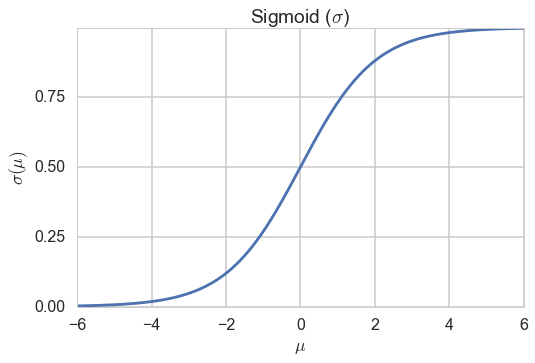
\includegraphics[scale=0.5]{sigmoid}
\end{figure*}


\noin The \textit{hypothesis}, $h_\theta(\boldx)$ given the weights $\theta$, is defined as
\begin{align*}
h_\theta(\boldx) &= \sigma(\theta^T\boldx) = \sigma \Big(\sum_{i=1}^n \theta_i \boldx_i \Big) \\ 
\Pr(y | \boldx, \theta) &= \Bern(y | h_\theta(\boldx))
\end{align*}

\noin Finally, $y$ is mapped to the discrete binary set $\{0, 1\}$ using a decision boundary $d$, where $0 \leq d \leq 1$.
\begin{align*}
h_\theta(\boldx) \geq d &\to y = 1 \\
h_\theta(\boldx) < d &\to y = 0 \\
\end{align*}

\noin Based on training data, a logistic regression model learns to optimize its predictions for newly observed data by updating the weights $\theta$. The weights in $\theta$ can be thought of as the control gates for the flow of information, and increasing the value of weight represents an increase in the importance of that information. In order to make the parameter update, a cost function $J$ is used to generate an error metric for the predicted outcome $h_\theta(\boldx)$ based on the "correct" observed outcome $\boldy$ for each observation-outcome pair in the training data. $\theta$ is then updated based on $J(\theta)$ by a method known as stochastic gradient descent (SGD), which is not discussed further here. The ultimate objective, using SGD, is to minimize the cost $J(\theta)$ over the training data. 
$$J(\theta) = \frac{1}{m} \sum_{\boldx} Cost(h_\theta(\boldx), \boldy)$$
So the optimal parameters $\hat{\theta}$ are $$\hat{\theta} = \argmin_\theta J(\theta | \mathcal{X}, \mathcal{Y})$$

Multinomial logistic regression is a generalization of logistic regression to the case where we want to classify data into $K$ classes, not just two. The objective is to develop a hypothesis to estimate $\Pr(\boldy = k | \boldx)$ for $k \in 1, \ldots, K$. This is useful in handwritten digit recognition, for example, where $\boldx$ is a numerical representation of an image, and $h_\theta(\boldx)$ describes the probability that the image represents a specific digit for all digits 0-9 ($K=10$). $\argmax_k h_\theta(\boldx)$ therefore tells us which digit is most likely represented in the image. \\

In order to represent $K$ classes, $\theta$ is now a \textit{matrix} of weights, making $\theta^T\boldx$ an activation \textit{vector}. The sigmoid function is replaced with the softmax, which generalizes the sigmoid function and normalizes the activation vector such that the resulting vector represents a probability distribution over the $K$ classes. Since $h_\theta(x)$ is a distribution, its elements must sum to 1.

$$h_\theta(\boldx) = \begin{bmatrix}
			P(\boldy = 1| \boldx, \theta) \\
			P(\boldy = 2| \boldx, \theta) \\
			\vdots \\
			P(\boldy = K| \boldx, \theta) \\
			\end{bmatrix}
			= \frac{1}{\sum_{i=1}^K \exp(\theta^{(i)T}\boldx)}
			\cdot \begin{bmatrix}
			\exp(\theta^{(1)T}\boldx) \\
			\exp(\theta^{(2)T}\boldx) \\
			\vdots \\
			\exp(\theta^{(K)T}\boldx) \\
			\end{bmatrix}$$ \\
			
\noin where $\theta$ is represented as

$$\theta = \begin{bmatrix} | && | && | && | \\
		\theta_1 && \theta_2 && \ldots && \theta_K \\ 
		 | && | && | && |
		\end{bmatrix}$$ \\

The most likely classification is therefore $$\argmax_k Pr(\boldy = k| \boldx, \theta)$$


\subsection*{Neural Networks}

In this section, we introduce \textit{artificial neural networks}, a family of machine learning models that are the focus of this thesis. Neural networks give us a way to model deeper interactions, and to generate predictions based on a combination of many non-linear functions - a series of cascading smaller decisions to determine a larger decision. They are exceptionally powerful, and by the Universal Approximation Theorem (Cybenko et. al. 1989), a feed-forward 3-layer neural network of finite size is proven to approximate any continuous function bounded by $n$ dimensions with any desired non-zero error \citep{goldberg2015nnlp}. As in multinomial logistic regression, the objective is $K-class$ classification. Neural networks are loosely inspired by the architecture of biological neural networks, where the complex decisions computed by our brains is a function of the many, small computations made by individual neurons. In an artificial network, the "neuron" is a unit with a unique weight that accepts a vector input and returns a scalar output. Neurons are organized as a series of layers, where the first is referred to as the "input" layer, the intermediary layers being the "hidden" layer, and the final layer being the "output" layer. In order to obtain the $K$-class distribution, $\boldx$ is "fed forward" through the network by a process known as forward propagation. The process is shown below for a 3-layer network, where $\sigma$ is the sigmoid function (applied element wise). $\theta^{(i)}$ is the matrix of parameters that control the mapping of input units to hidden units for the $i$th layers. $\boldb^{(i)}$ is the bias neuron for the $i$th layer. $L_i$ is the size of the $i$th layer.
\begin{align*}
\boldz^{(1)} &= \theta^{(1)T}\boldx + \boldb^{(1)} \\
\bolda^{(1)} &= \sigma(\boldz^{(1)}) \\
\boldz^{(2)} &= \theta^{(2)T}\bolda^{(1)} + \boldb^{(2)} \\
\bolda^{(2)} &= \sigma(\boldz^{(2)}) \\
\boldz^{(2)} &= \theta^{(3)T} \bolda^{(2)} \\
h_{\theta}(\boldx) &= \sigma(\boldz^{(3)})
\end{align*}

where $$x \in \reals^m, h_{\theta}(\boldx) \in \reals^K, \theta^{(i)} \in \reals^{L_{i} \times L_{i+1}}, b^{(i)} \in $$

When a layer is reached, each neuron in the layer performs a linear combination of the input and its parameters, applies a non-linear function (i.e. sigmoid $\sigma$), and then passes the result forward to each neuron in the next layer. Each connection between two neurons also carries a separate, adjustable parameter. This continues until the final layer, where the output layer returns a vector that is forwarded through a softmax function to obtain the $K$-dimensional distribution $h_{\theta}(\boldx)$.

\begin{figure*}[h]
\caption{Abstract representation of a three-layer neural network architecture, where each circle represents a neuron. $\theta$ controls the flow of information between activation layers.}
\centering
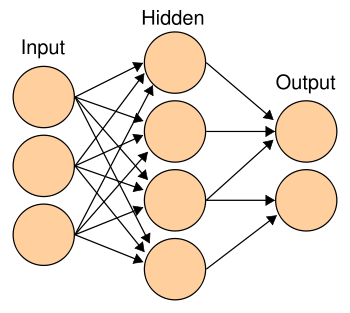
\includegraphics[scale=0.55]{nn}
\end{figure*}

For all neural models used in this thesis, the objective is to minimize \textit{negative log likelihood}. Likelihood ($\mathcal{L}$) is a function of the parameters $\theta$ given a set of observations $\mathcal{X}$, and it is in fact equivalent to the probability of those observations given the parameters.
$$\mathcal{L}(\theta | \mathcal{X}) = P(\mathcal{X} | \theta)$$
For mathematical ease, log likelihood is used.
$$\log \mathcal{L} = \log \prod_{i=1}^{m} h(\boldx_i | \theta) = \sum_{i=1}^{m} h(\boldx_i | \theta)$$
And maximizing log likelihood is equivalent to minimizing negative likelihood.
$$\hat{\theta} = \argmax_{\theta} \sum_{i=1}^{m} h(\boldx_i | \theta) = \argmin_{\theta} \Big[- \sum_{i=1}^{m} h(\boldx_i | \theta)\Big]$$

The parameters $\theta$ are updated by calculating $J(\theta)$ and computing the partial derivatives (the "gradients") of $J(\theta)$ with respect to each of the parameters. 
$$\theta_{j} = \theta_{j} - \alpha \frac{\partial J(\theta)}{\partial \theta_j}$$
The partial derivatives of $J$, or the gradient vectors, describe the direction of \textit{steepest ascent} of $J(\theta)$. So by subtracting these gradients at each update, the network descends towards a minimization of $J$. The learning rate, $\alpha$, adds a multiplicative factor that controls the strength of each gradient update. This process of passing gradients through the network and updating $\theta$ is known as backwards propagation.



\subsection*{Recurrent neural networks (RNNs) and sequential data}

An important limitation of "vanilla" neural networks, like the ones described in the previous section, is that they treat each input independently of all other inputs. In supervised learning tasks where the input data is in the form of \textit{sequences}, recurrent neural networks (RNNs) are an effective model because of their ability to "remember" features of recent computations. Formally, a sequence of data is defined as a series of input vectors over a discrete set of time-steps, such that $\boldx_i$ is the input vector at time step $i$. RNNs can train very effectively on datasets even when the inputs lack a naturally sequential order (\cite{karpathy2015rnn}).\\

At each time step, the recurrent model receives two inputs, the feature vector $x_t$ as well as the output of the hidden layer from the previous time step $s_{t}$. During forward propagation, an RNN internally stores the output of each hidden layer and returns a distribution for the next time step, $h_{t+1}$. The most basic RNN architecture, known as the Elman network \citep[p.~56]{goldberg2015nnlp}, can be modeled as follows:
\begin{align*}
\bolda_i(\boldx) &= \sigma(\theta^{(1)T}\boldx_i + \theta^{(2)T}\boldy(\boldx_{i-1})) \\
\boldy(\boldx_i) &= g(\bolda_i(\boldx))
\end{align*}
where $$\theta^{(1)} \in \reals^{|\boldx| \times h}, \theta^{(2)} \in \reals^{h \times h}$$

\noin and $g$ is a non-linear transformation, such sigmoid ($\sigma$) or tanh. Note that the parameters $\theta$ can be updated in the middle of forward propagation over a sequence, or after the entire sequence has been fed through. Training an RNN follows the same procedure as the non-recurrent model - create a computation graph over time, calculate error for the most recent prediction, and then back-propagate the error across the unfolded network, generating gradients and updating each weight in $\theta$ \citep[p.~63]{goldberg2015nnlp}. \\

\begin{figure*}[h]
\centering
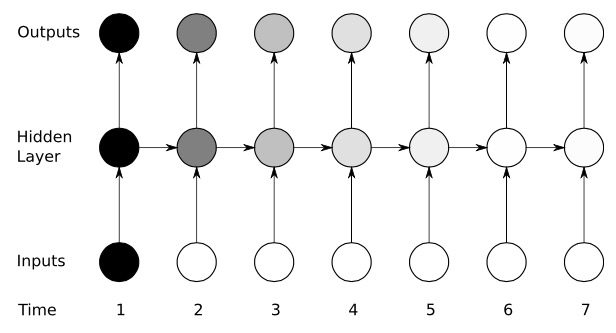
\includegraphics[scale=0.55]{rnn}
\caption{Abstraction of an RNN over a time series. The activation of the neurons in the hidden layer is a function of the input from the previous layer and its own output from the previous computation. }
\end{figure*}

The recurrent model of incorporating feedback from previous decisions is a promising approach to the harmonization task, where the chorale can be represented as a sequence of melody notes with corresponding, interrelated harmonizations. \cite{karpathy2015rnn} famously cited the "unreasonable effectiveness" of recurrent neural networks in learning sequential data for a variety of tasks, including speech recognition, language translation, and image captioning. As a result, we hypothesized that recurrent models would perform particularly well on musical tasks that require contextualized decision-making and benefit from correlating temporally distant inputs.

\subsection*{Improving the recurrent model: Long Short-Term Memory networks}

Long Short-Term Memory networks (LSTMs) are a variant of RNNs that replace the hidden layer neurons with specialized cells for enhanced memory capabilities, first introduced by Schmidhuber and Hochreiter in 1997. In the original RNN architecture, the feedback is "short-term" in that $s_t$ is only a function of the input at time $t-1$ (and much more weakly for previous time steps). Therefore as the sequence is fed through the network, the signal from earlier time-steps is gradually lost. This phenomenon is known as the "vanishing gradients problem" \citep[p.~56]{goldberg2015nnlp} and it constitutes a major drawback to using the original RNN architecture. LSTMs solve this long-term dependency issue by substituting the regular neuron with a \textit{memory cell} that can retain much more distant signals from previous inputs. Information is stored and segregated within the cell by use of multiplicative gate units, such as input, forget, and output gates. These gates allow information to flow through the cell without affecting other memory contents, while also deciding what cell  information should be kept versus overwritten by newer signals. A gate $\boldg$ is represented as a $n$-dimensional one-hot vector, and the values of $\boldg$ are considered parameters of the model. A value of 1 in a gate has the effect of retaining its corresponding signal element, while a value of 0 effectively eliminates that element. The deeper mathematical foundations for LSTMs are not necessary to understand, but they have proven to be exceptionally effective models, designed specifically for retaining information over long periods of time. When applied to music, LSTMs have proven effective at learning global musical structures and generating melodies \citep{eck2002blues}.

\begin{figure*}[h]
\centering
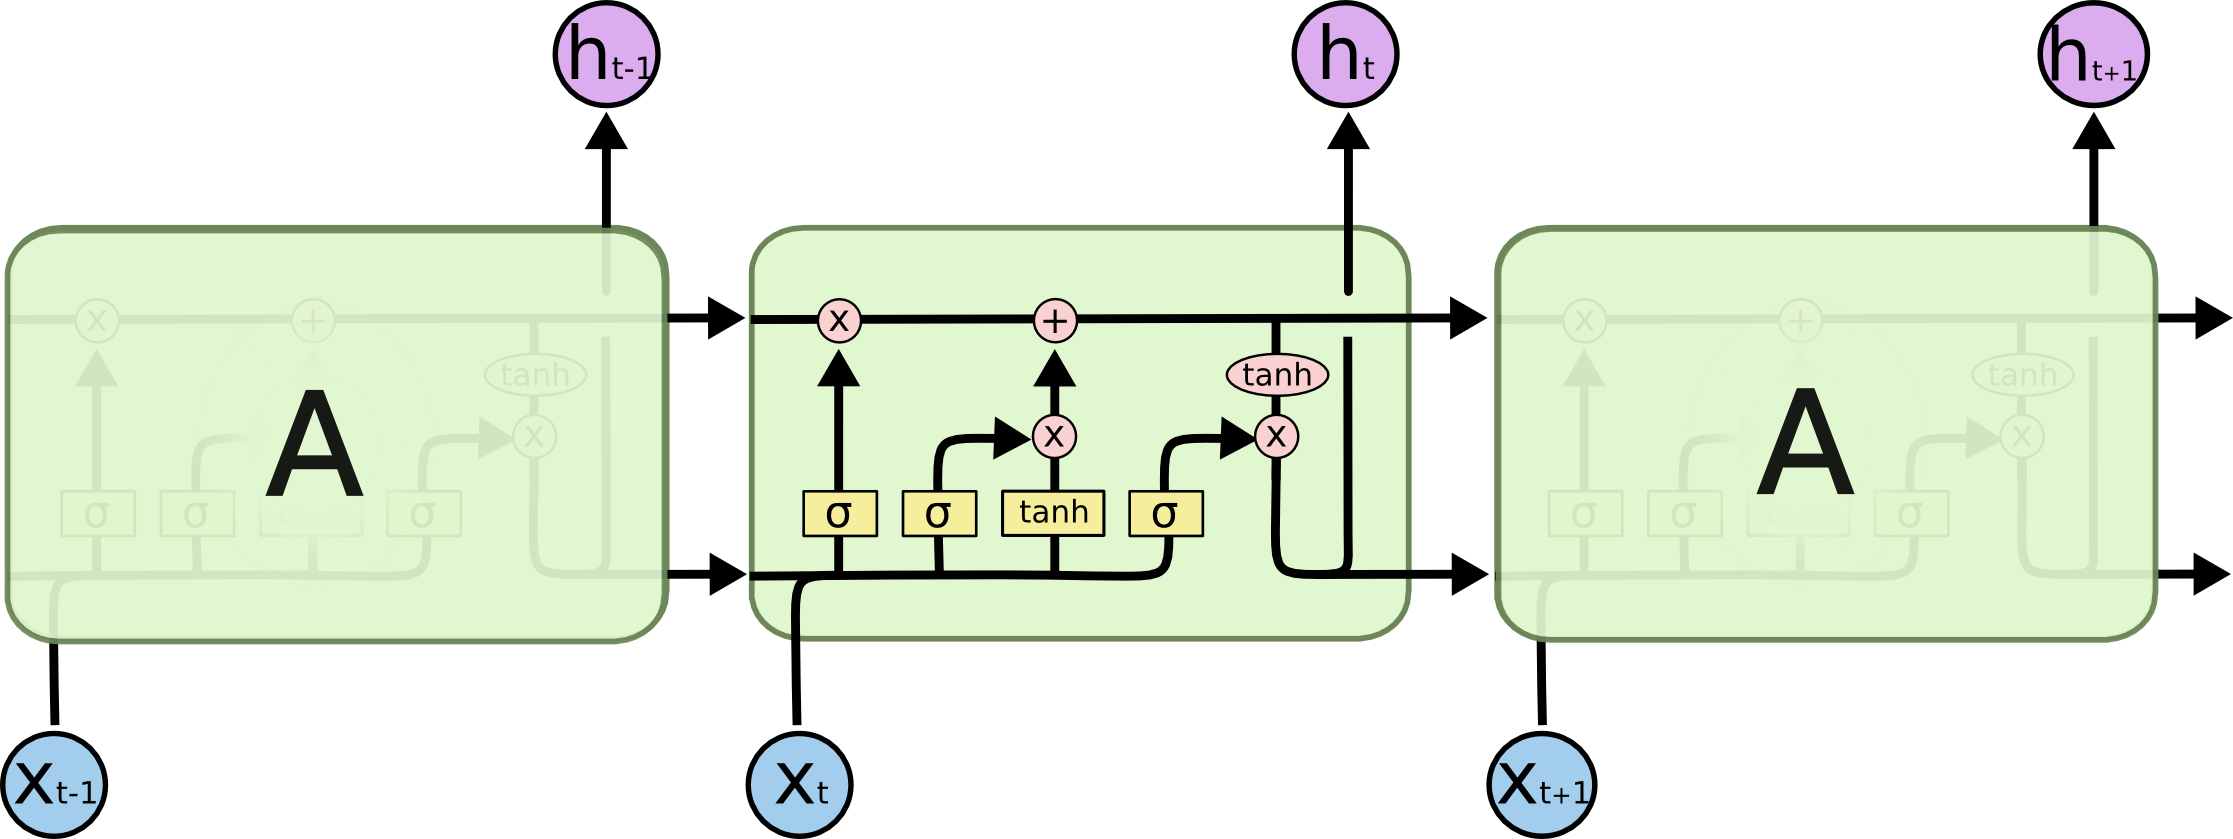
\includegraphics[scale=0.5]{lstm2}
\caption{The chained structure of an LSTM memory cell. Each cell contains multiple network layers, where the RNN presented previously has only one (the sigmoid layer). Diagram borrowed from \citet{colah2015lstms}.}
\end{figure*}



%%%%%%%%%%
%-----------------------
%%%%%%%%%%

\section{An introduction to tonal harmony and the chorale}

The primary objective of this thesis is to train a variety of models on the four-voice chorales composed by J.S. Bach in order to learn the task of chorale harmonization. However, each model is not given an actual musical score as input, but rather a numerical representation of "features" extracted from the score. Features are variables that describe some aspect of the data, and a thoughtful selection of features is one of the largest factors in having the model learn effectively. The features selected from the chorales include both score-wide features, such as the key signature, as well as local features that describe the melody at a specific moment in numerical terms, such as the beat strength of the melody note. In order to understand the meaning of the musical features selected from the chorales and their significance in learning the task of harmonization, a tailored overview of tonal harmony and the properties of the chorales is provided here. Musical properties are described as computational objects to illustrate the ability to translate between these properties and numerical representation. \\

\subsection*{Pitch class, pitch, note}

The fundamental musical object in Western tonal music is the \textit{pitch class}. The tonal system operates over a series of 12 \textit{pitch classes}, and some pitch classes (i.e. C$\sharp$/D$\flat$) are referred to by different names depending on the current context. A pitch class is defined by its unique index - a integer between 1 and 12. It is common to assign the tonic pitch class as 1, the pitch class above it as 2, and so on.

\begin{center}
C, C$\sharp$/D$\flat$, D, D$\sharp$/E$\flat$, E, F, F$\sharp$/G$\flat$, G, G$\sharp$/A$\flat$, A, A$\sharp$/B$\flat$, B
\end{center}

A \textit{pitch} is an object defined by a pitch class and an octave, identifying a unique frequency. A common representation of pitch is MIDI (Musical Instrument Digital Interface) notation, which today remains the most widely used protocol for communication of musical information between electronic instruments. In MIDI, a pitch is identified by a unique integer between 21 and 108 (inclusive). However, a disadvantage to MIDI is that it conflates enharmonic pitches (i.e. C$\sharp$5 has the same MIDI value as D$\flat$5), so information about the function of a pitch within a key signature is lost with this representation. \\

We then define a \textit{note} as a pitch with the additional feature of duration.

\subsection*{Scale, chord, key}

The musical objects defined here are fundamental indicators of harmonic information. A \textit{scale} is an ordered collection of pitch classes defined by an initial pitch class and a quality - major or minor - that defines the intervals between each note in the collection. Each pitch class in the scale is given an indexed scale degree and a name. The two most important elements in the scale are the "tonic" ($\hat{1}$) and "dominant" ($\hat{5}$). But more generally, a melody over a scale is guided by the characteristic tension or stability of the scale's pitch classes. The "tonic" represents the ultimate point of stability, whereas the leading tone ($\hat{7}$) creates a sense of motion towards the tonic. Therefore, pitch is a crucial feature in predicting the continuation of a melody or the harmonization of an existing melody. \\

The strong parallel between scales and chords can be defined as a \textit{chord-scale duality}. A \textit{chord} is a collection of three or more notes sounded together. The pitches that comprise a chord imply a scale that contains those pitches; and similarly, a scale implies the set of \textit{triads} that can be constructed starting from each note of the scale. \\

The \textit{key} of a piece is a combination of two pieces of harmonic information - the tonic pitch class, and the chord (or scale) that represents full harmonic resolution. In major and minor keys, this chord is a \textit{triad}, which in the key of C major is the pitch class set \{C, E, G\}. The triad alone is able to define the diatonic scale for the piece, which is represented symbolically as a key signature that specifies the pitch classes of the diatonic scale.

\begin{figure*}[h]
\centering
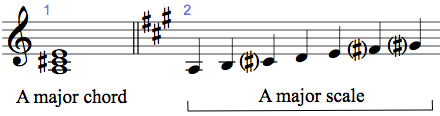
\includegraphics[scale=0.6]{chord-scale}
\caption{chord-scale duality.}
\end{figure*}


\subsection*{Harmonic analysis and motion}

When harmonizing a chorale, an important first step is to analyze the chorale melody and determine the chord progression that the harmonizing voices will imply. A standard approach for notating chord progressions in classical harmony is Roman numeral analysis. Roman numeral analysis describes a harmony by assigning a Roman numeral based on the chord root and a uppercase or lowercase version (i.e. \rom{2} vs. \lrom{2}) based on the chord quality. Superscripts are used to denote chord inversions, indicating which pitch class in the chord appears in the lowest voice \citep[pg.~68-9]{laitz2008}. For example, in the key of A major, the A major triad \{A, C$\sharp$, E\} is assigned \rom{1} and an E dominant 7th chord \{E, G$\sharp$, B, D\} is assigned \rom{5}$^7$ based on the E major triad, notated as \rom{5}. Roman numeral analysis is powerful because it focuses on the harmonic information stored in triads. The motion between tonic and dominant triads alone can firmly establish a key, as well as a sense of tension and resolution that is generated by harmonic motion away from and towards the tonic harmony \citep[pg.~106]{laitz2008}. \\

In performing Roman numeral analysis, context is a crucial factor because each harmony is analyzed with respect to the key of the chorale as well as the harmonies that preceded it. This is why harmonies are often described as a progression, or \textit{sequence}. The ordering of harmonies - like the ordering of words in a sentence - is a essential feature of a harmonic progression, and an important feature to consider when constructing models to generate new progressions. \\

\textit{Cadences} are the components of a harmonic progression that conclude a musical phrase or section. They are important harmonic indicators that lead to a point of a resolution or heightened tension, depending on the type of cadence, and as a result they control the flow of the music. Statistically, the ability of a model to accurately predict the location and quality of a cadence can serve a useful qualitative indicator of a model's performance because cadences are the most defining feature of a harmonic progression. \\


\subsection*{Bach's settings of the chorales}

A \textit{chorale} is a congregational hymn that first came into use during the early decades of the German Protestant Reformation, under Martin Luther. These hymns were originally composed as a one-voice melody with lyrical text, and composers of the time drew heavily (and sometimes borrowed verbatim) from existing secular songs, medieval Gregorian chant, and other sacred works when writing new chorales. In the Baroque era, the composer Johann Sebastian Bach revived the chorale tradition and composed several new chorale melodies. However, his most lasting contribution to the chorale form remains his harmonizations of hundreds of chorales, which were inserted into many of his larger vocal and instrumental compositions, including the St. Matthew Passion and the cantatas \citep{leaverchorale}. His harmonization of four-voice chorales - of which 341 exist in the Riemenschneider collection - are masterful studies in four-voice counterpoint, and they remain a guide for modern church musicians, jazz writers, arrangers and students alike. This corpus established fundamental conventions for tonal harmony with respect to voice leading, cadential movement, and intervallic relationships between voices. \\

Structurally, the chorale is written for the four standard voice ranges: soprano, alto, tenor, and bass. The original chorale melody is sung by the soprano, while the lower voices collectively embody the \textit{harmonization} of the melody. It closely resembles the chordal motion of the modern sacred hymn, and the rhythmic complexity of the chorales is intentionally minimal in order to draw focus to the harmonic motion taking place on each beat. The entire chorale is segmented into shorter phrases by a series of \textit{fermatas} that indicate a pause and point of emphasis. The fermata denotes a point of cadence where a point of tension or resolution is firmly established. \\

The chorale should be viewed in multiple dimensions. In the vertical dimension, the notes of each voice at time $t$ can be heard simultaneously as a chord; and therefore, the chorale can be abstracted to a four-voice chordal progression. Learning to recognize and generate choral progressions is the primary task of models of this thesis. The progression is guided by the cadences that structure each phrase, and each cadence is defined by the relationship between the melody and the bass line. The inner voices (alto and tenor) function as supportive voices that "fill out" the harmonies. However, in the linear dimension, the chorale represents a combination of four independent but complimentary melodic lines, and the contour of each line is governed by the conventions of \textit{voice leading}. Voice leading embodies a broad set of characteristics, but they include rules about preferred and undesired intervals, parallel and contrary motion, and methods for rhythmically embellishing a chord progression (i.e. passing tones). The conventions of voice leading the acceptable motion in each voice as the harmony shifts in the vertical dimension. \\

\begin{figure*}[h]
\caption{ The opening of the chorale \textit{Nun lob' mein' Seel', den Herren} }
\centerline{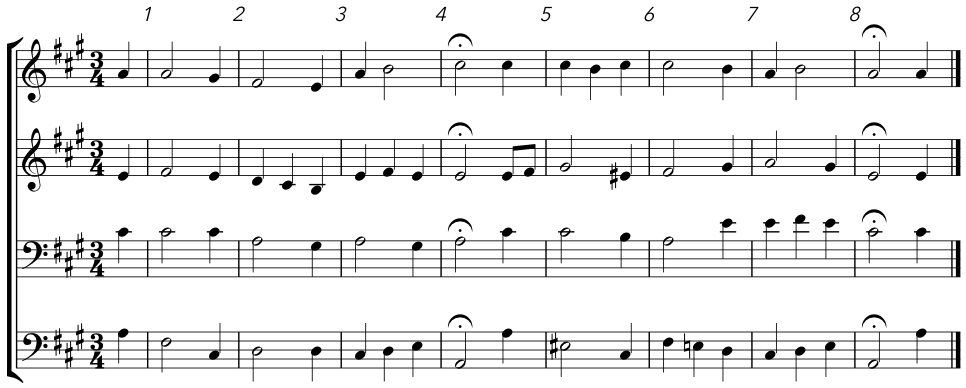
\includegraphics[scale=0.45]{chorale_mine}}
\end{figure*}

The opening phrases of the chorale \textit{Nun lob' mein' Seel', den Herren} illustrate the importance of context in the task of harmonization. An important property of Bach's four-voice chorales is that the harmonic transitions occur very uniformly on each beat, so the task of harmonizing a chorale can be into divided into a time series of decisions for each beat of the melody. Bach's choice of harmonization for each beat is not a localized decision, but rather a decision that factors in information about the harmonic progression that preceded the current moment as well as the likely harmonies to occur next. For example, in measures 3-4 and measures 7-8, Bach constructs the cadence \lrom{2}$^6$ - \rom{5} - \rom{1}. Were we harmonizing the chorale ourselves in the same way and decided to harmonize the melody with a \lrom{2}$^6$ voicing on beat 2, this constrains the harmonies we could convincingly assign to beat 3. An additional constraint is placed by the fermata that occurs two beats later, which is almost certainly the resolution point of an authentic (\rom{1}) or half (\rom{5}) cadence. The harmonization of beat 3 must therefore bridge its surrounding harmonies to satisfy the expression \lrom{2}$^6$ - * - \{\rom{1}, \rom{5}\}. \\ 

Another important harmonic choice to examine is the C$\sharp^7$ harmony in measure 5, which is not diatonic to the chorale's key of A-major. In this case, C$\sharp^7$ functions as a secondary dominant, since the harmony resolves to $F\sharp$-minor in measure 6, and in f$\sharp$, C$\sharp^7$ is the dominant 7th chord. Secondary dominants are an effective tool for prolonging the resolution towards a certain harmony, and Bach uses them frequently to expand his harmonic pallette. The chorale \textit{Warum betr�bst du dich, mein Herz} illustrates the use of secondary dominants to facilitate a chromatically ascending bass line. \footnote{This is not my diagram, but will be replaced with my own (and my own Roman numeral analysis). Current image credited to \url{https://lukedahn.wordpress.com/2010/02/08/bachs-12-tone-chorale-phrases/}.} \\

\begin{figure*}[h]
\caption{ First phrase of \textit{Warum betr�bst du dich, mein Herz} }
\centerline{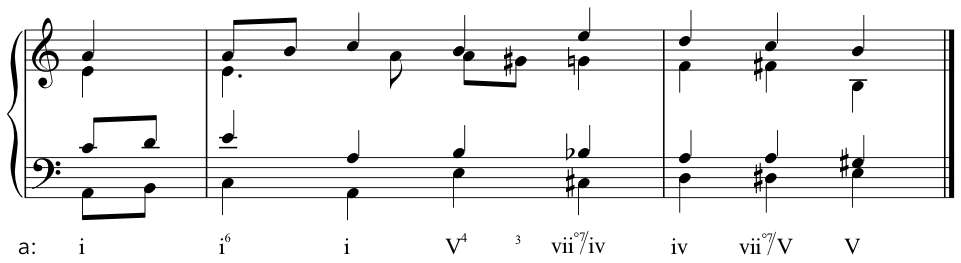
\includegraphics[scale=0.45]{chorale2_mine}}
\end{figure*}

Therefore, a substantial model for chorale harmonization requires a variety of past, present, and future information in order to make accurate decisions. Characteristics of the melody note - such as pitch, beat strength, or the presence of a fermata - provide information about the stability of the harmony and whether or not a transitional harmony is more appropriate (such as a secondary dominant). The preceding harmonies indicate whether larger harmonic progressions are taking place, such as cadences and prolongations of a single harmony. And information about future events like fermatas or the final beat signal the endpoint of the current phrase, and so a convincing harmonic progression should lead towards the point of resolution. \\

\citet{cross2008} discuss the potential for statistical learning over the chorales as a dataset. They present a formal mathematical approach for segmenting chorales into segments of a quarter note. The approach to "quantizing" the chorales discussed in Chapter 2 loosely follows these concepts but relies on a set of rules based on prior musical knowledge. Moreover, the study describes the unbalanced distribution of chords in the corpus. In their dataset, tonic and dominant chords occurred 5285 times, while all other chords collectively occur 5604 times. As a result, we hypothesized that harmonic classification for certain models might suffer from an imbalanced dataset. The imbalance in chord frequency translates to an imbalance in chord transition, and as might be suspected, the frequency of transitions between \rom{1}, \rom{4}, and \rom{5} harmonies clearly dominate. As a result, there are many chords that occur with relative infrequency that may be difficult to classify. \\

A final potential difficulty to note is that chorales can be harmonized in many different ways. we intentionally kept chorales in the dataset that shared melodies but had different harmonizations in order to preserve the complexity of the task, which should be reflected in the results.

\newpage

\printbibliography









\end{document}